% Chapter 1

\chapter{Introducción General} % Main chapter title

\label{Chapter1} % For referencing the chapter elsewhere, use \ref{Chapter1} 
\label{IntroGeneral}

%----------------------------------------------------------------------------------------

% Define some commands to keep the formatting separated from the content 
\newcommand{\keyword}[1]{\textbf{#1}}
\newcommand{\tabhead}[1]{\textbf{#1}}
\newcommand{\code}[1]{\texttt{#1}}
\newcommand{\file}[1]{\texttt{\bfseries#1}}
\newcommand{\option}[1]{\texttt{\itshape#1}}
\newcommand{\grados}{$^{\circ}$}

%----------------------------------------------------------------------------------------
La idea de esta sección es presentar el tema de modo que cualquier persona que no conoce el tema pueda entender de qué se trata y por qué es importante realizar este trabajo y cuál es su impacto.

\section{Motivación}

\section{Soluciones comerciles existentes}

\section{Objetivos}


\begin{figure}[h]
	\centering
	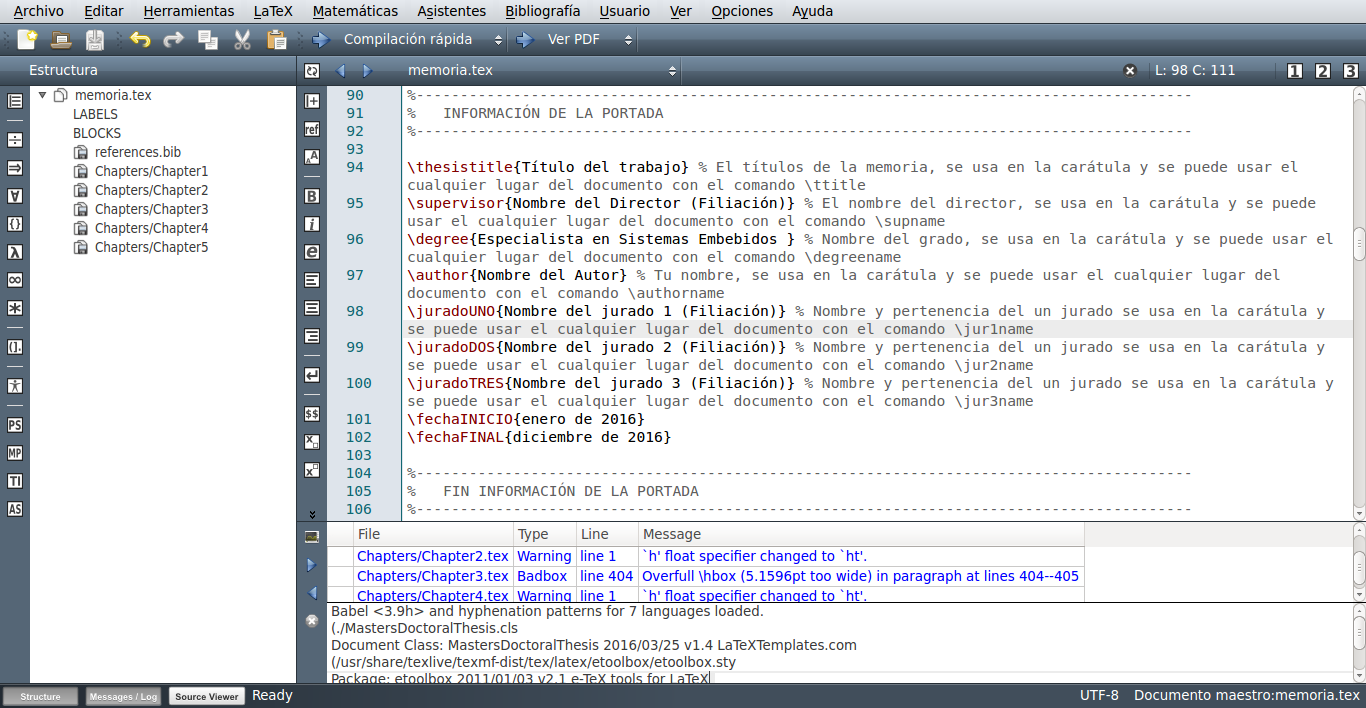
\includegraphics[width=\textwidth]{./Figures/texmaker.png}
	\caption{Entorno de trabajo del texMaker.}
	\label{fig:texmaker}
\end{figure}


%----------------------------------------------------------------------------------------






